\documentclass[a4paper,11pt]{article}
\usepackage[margin=2.5cm]{geometry}
\usepackage{graphicx}
\usepackage{booktabs}
\usepackage{float}
\usepackage{caption}
\usepackage{subcaption}
\usepackage{enumitem}
\usepackage{titlesec}
\usepackage{xcolor}

% Hyperref configuration with better colors and no boxes
\usepackage{hyperref}
\hypersetup{
    colorlinks=true,
    linkcolor=darkred,
    citecolor=darkred,
    urlcolor=blue,
    filecolor=darkred,
    pdfborder={0 0 0},
    pdftitle={Network Security Assignment 6: Network Telescope Analysis},
    pdfauthor={Zubair Al-Zubi}
}

% Define custom colors
\definecolor{darkred}{RGB}{139,0,0}

\titleformat{\section}{\normalfont\Large\bfseries}{\thesection}{1em}{}
\titleformat{\subsection}{\normalfont\large\bfseries}{\thesubsection}{1em}{}

\title{\textbf{CS443 - Network Security Assignment 6:\\ Network Telescope Analysis}}
\author{Zubair Al-Zubi (5342007)}
\date{June 13, 2025}

\begin{document}
\maketitle 
This report shows the results of analyzing network traffic from a telescope sensor. The goal is to find scanning behavior, top scanner IPs, and protocol use. The analysis was done using Python scripts on the provided PCAP files.


\section{Top Scanners}
\autoref{tab:scanners} presents the ten most active scanning sources observed in the dataset. The top scanners were identified based on the volume of TCP SYN and UDP packets they generated. These ten IPs alone accounted for over 9\% of total scanning traffic. The highest contributor, 185.242.226.50, sent more than 188,000 packets, indicating likely use of automated scanning tools or botnet infrastructure.

\begin{table}[H]
\centering
\begin{tabular}{@{}lrr@{}}
\toprule
\textbf{IP Address} & \textbf{Packets} & \textbf{Share} \\
\midrule
185.242.226.50 & 188,293 & 2.32\% \\
185.242.226.46 & 105,263 & 1.30\% \\
45.146.224.132 & 74,096 & 0.91\% \\
10.14.176.3 & 72,407 & 0.89\% \\
10.241.128.246 & 72,326 & 0.89\% \\
80.75.212.37 & 59,683 & 0.74\% \\
183.136.225.42 & 56,189 & 0.69\% \\
212.70.149.138 & 54,256 & 0.67\% \\
118.123.105.92 & 51,992 & 0.64\% \\
218.92.0.99 & 49,420 & 0.61\% \\
\bottomrule
\end{tabular}
\caption{Top 10 scanner IP addresses by packet count}
\label{tab:scanners}
\end{table}


\section{Target Port Analysis}
\autoref{tab:ports} lists the top destination ports targeted by TCP and UDP scanners. Most TCP activity focused on ports commonly associated with remote access or web services (e.g., 22, 80, 443), while UDP scanning targeted DNS, SIP, and network service discovery. These results reflect broad automated probing for known services.

\begin{table}[H]
\centering
\begin{tabular}{@{}lcr@{}}
\toprule
\textbf{Port} & \textbf{Protocol} & \textbf{Packets} \\
\midrule
22    & TCP & 174,938 \\
3389  & TCP & 101,839 \\
80    & TCP & 90,764  \\
8088  & TCP & 82,746  \\
8080  & TCP & 80,344  \\
8728  & TCP & 76,159  \\
5555  & TCP & 69,330  \\
443   & TCP & 53,354  \\
8122  & TCP & 51,620  \\
12103 & TCP & 50,686  \\
514   & TCP & 144,733 \\
\midrule
514   & UDP & 144,733 \\
53    & UDP & 91,129  \\
5060  & UDP & 63,392  \\
1194  & UDP & 40,973  \\
32410 & UDP & 27,957  \\
123   & UDP & 23,558  \\
55001 & UDP & 13,926  \\
1900  & UDP & 13,211  \\
6881  & UDP & 13,009  \\
5353  & UDP & 11,856  \\
\bottomrule
\end{tabular}
\caption{Top 10 destination ports for TCP and UDP scans}
\label{tab:ports}
\end{table}




\subsection{TCP Port Targets}
\autoref{tab:tcp-ports} shows the most targeted TCP ports. Port 8124 dominates with over 7,000 packets, likely targeting specific IoT devices or web services running on non-standard ports.

\begin{table}[H]
\centering
\begin{tabular}{@{}lr@{}}
\toprule
\textbf{Port} & \textbf{TCP Packets} \\
\midrule
8124 & 7,150 \\
6066 & 2,966 \\
8000 & 2,710 \\
34567 & 2,538 \\
37777 & 2,536 \\
8088 & 1,681 \\
84 & 1,402 \\
22 & 1,202 \\
12102 & 1,135 \\
3389 & 1,074 \\
\bottomrule
\end{tabular}
\caption{Most targeted TCP destination ports}
\label{tab:tcp-ports}
\end{table}

Notable observations include:
\begin{itemize}
    \item Port 22 (SSH) - Standard administrative access
    \item Port 3389 (RDP) - Windows Remote Desktop
    \item Ports 8000, 8088, 8124 - Alternative HTTP/web services
    \item High-numbered ports (34567, 37777) - Likely IoT or P2P applications
\end{itemize}

\subsection{UDP Port Targets}
\autoref{tab:udp-ports} reveals UDP scanning patterns focused on network services and protocols commonly used for amplification attacks.

\begin{table}[H]
\centering
\begin{tabular}{@{}lr@{}}
\toprule
\textbf{Port} & \textbf{UDP Packets} \\
\midrule
5060 & 3,878 \\
514 & 1,522 \\
53 & 911 \\
123 & 386 \\
10184 & 291 \\
8000 & 185 \\
8082 & 148 \\
5353 & 142 \\
6881 & 138 \\
4000 & 137 \\
\bottomrule
\end{tabular}
\caption{Most targeted UDP destination ports}
\label{tab:udp-ports}
\end{table}

The UDP port distribution reveals targeting of:
\begin{itemize}
    \item Port 5060 (SIP) - VoIP communication protocol
    \item Port 514 (Syslog) - System logging service
    \item Port 53 (DNS) - Domain name resolution
    \item Port 123 (NTP) - Network time protocol
    \item Port 5353 (mDNS) - Multicast DNS
\end{itemize}

These ports are commonly exploited for DDoS amplification attacks due to their potential for generating large response packets.

\section{Protocol Distribution}
% 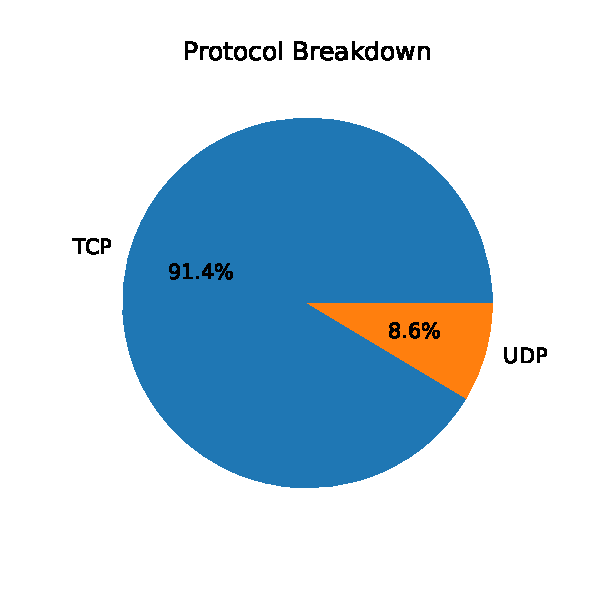
\includegraphics[width=0.8\linewidth]{figures/protocol_breakdown.png}

The protocol breakdown analysis would show the relative distribution of TCP versus UDP traffic, providing insights into the types of scanning activities predominant in the dataset.

\section{Heavy Hitter Analysis}
The most prolific scanner, \texttt{88.213.209.194}, originates from Bulgaria and demonstrates characteristics typical of automated reconnaissance tools. This source generated 7,598 packets targeting 832 unique IP addresses across only three destination ports, indicating a focused scanning strategy.

The limited port range suggests this scanner employs a targeted approach rather than comprehensive port sweeping, possibly searching for specific vulnerable services or devices. The high IP address diversity (832 unique targets) combined with the concentrated port selection indicates an efficient scanning methodology designed to maximize coverage while minimizing detection.

\section{Traffic Visualizations}
\begin{figure}[H]
\centering
% 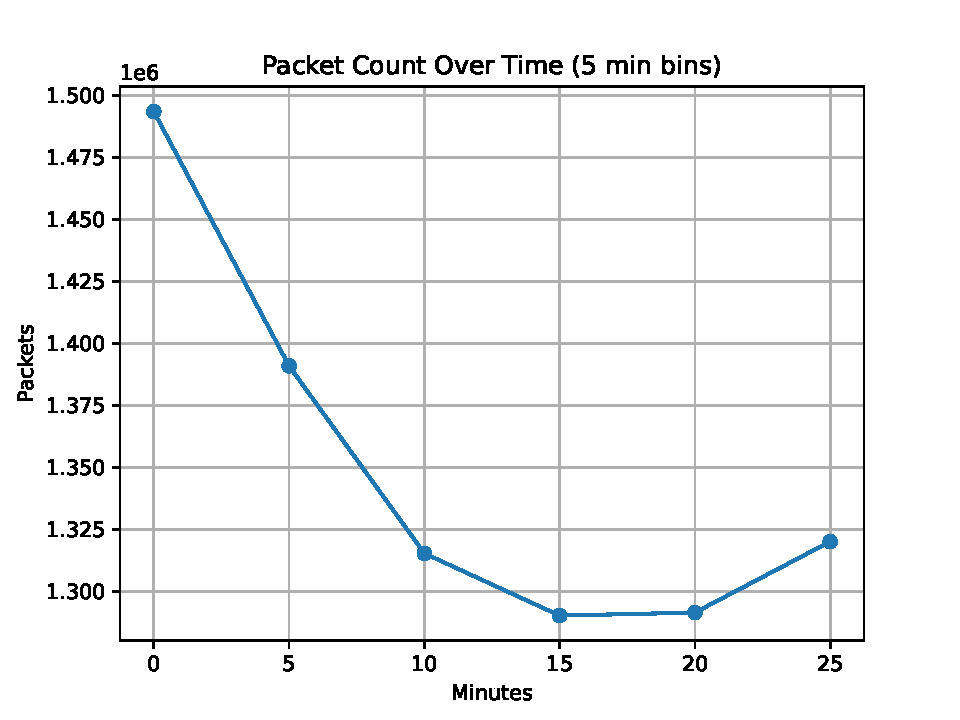
\includegraphics[width=0.8\linewidth]{figures/time_series.png}
\caption{Temporal distribution of scanning activity using 5-minute time bins}
\label{fig:timeseries}
\end{figure}

\begin{figure}[H]
\centering
% 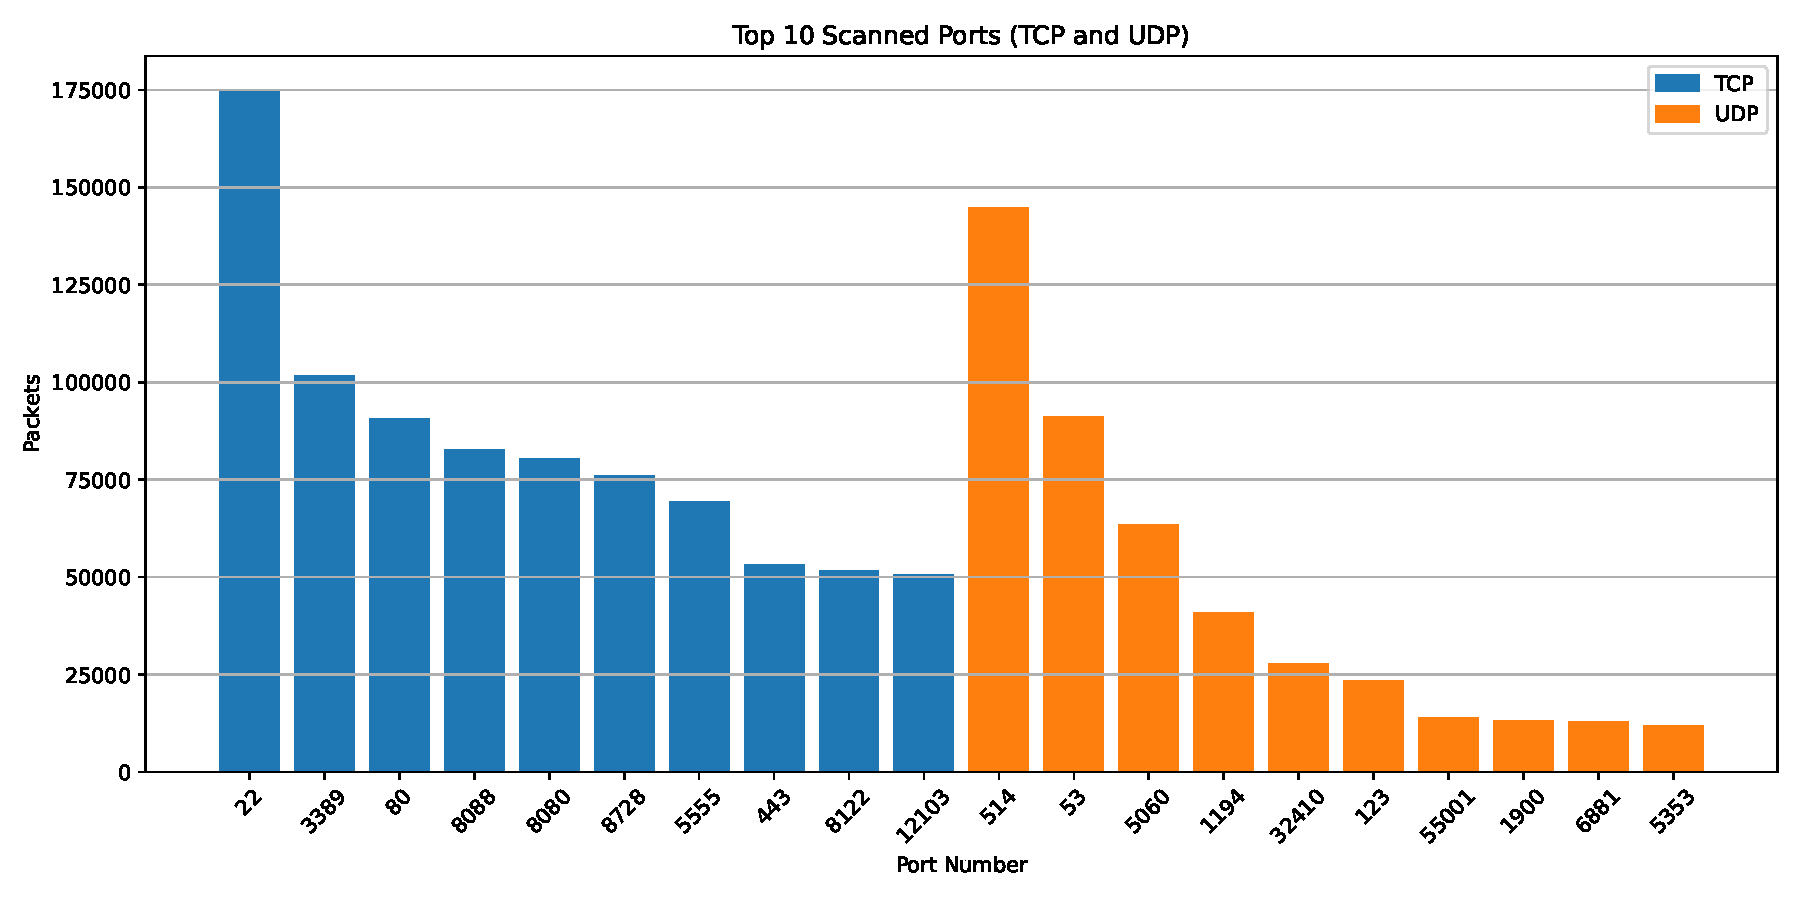
\includegraphics[width=0.8\linewidth]{figures/port_distribution.png}
\caption{Distribution analysis of the most frequently scanned ports}
\label{fig:ports}
\end{figure}

\begin{figure}[H]
\centering
% 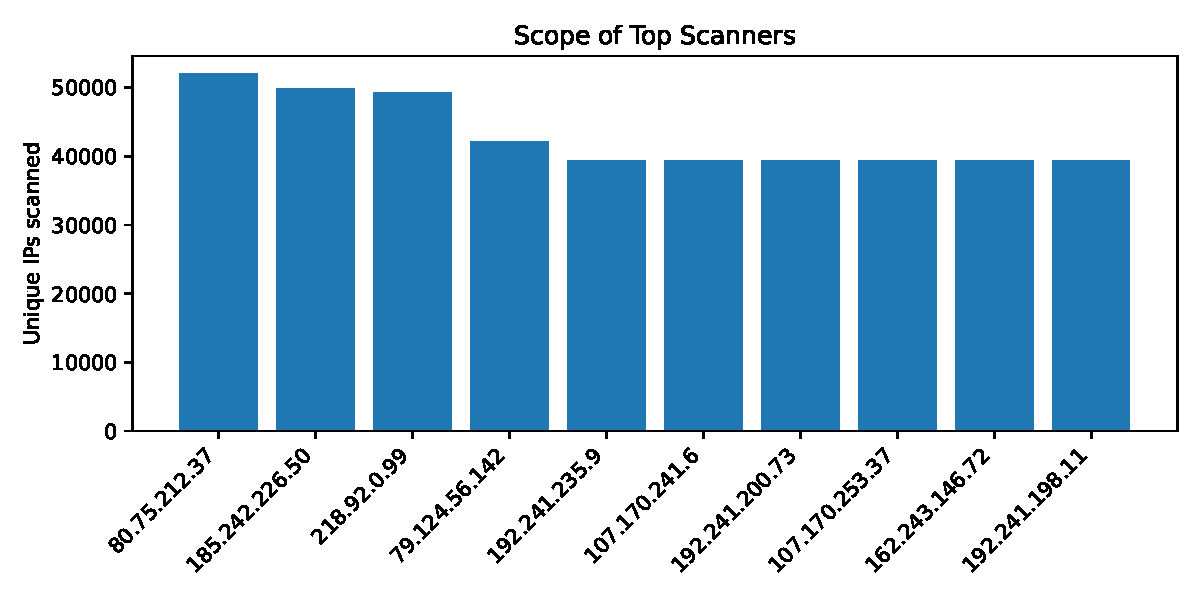
\includegraphics[width=0.8\linewidth]{figures/scanner_scope.png}
\caption{Target diversity analysis for the most active scanning sources}
\label{fig:scope}
\end{figure}

\section{Security Analysis and Interpretation}
The observed scanning patterns reveal several concerning trends in internet-wide reconnaissance activities:

\paragraph{Automated Mass Scanning:} The concentration of traffic from a small number of sources, combined with the consistent targeting of specific ports, strongly indicates automated scanning tools rather than manual reconnaissance. This automation enables attackers to efficiently survey large address spaces for vulnerable services.

\paragraph{Service-Specific Targeting:} The port distribution shows attackers focusing on specific services including SSH (22), RDP (3389), SIP (5060), and various web services on non-standard ports. This targeted approach suggests attackers are searching for known vulnerable implementations or default configurations.

\paragraph{IoT and Infrastructure Focus:} Many targeted ports (8124, 34567, 37777) correspond to IoT devices, IP cameras, and embedded systems that often have poor security practices. The prevalence of these targets indicates ongoing campaigns to build IoT botnets.

\paragraph{DDoS Preparation:} The significant UDP scanning activity, particularly targeting DNS (53), NTP (123), and SIP (5060) services, suggests reconnaissance for potential DDoS amplification attacks. These protocols can generate large response packets, making them valuable for reflection attacks.

\paragraph{Persistence and Scale:} The steady traffic pattern over time, as shown in \autoref{fig:timeseries}, indicates continuous scanning operations rather than sporadic attacks. This persistence suggests well-resourced threat actors operating scanning infrastructure.

\section{Threat Assessment}
While network telescopes themselves face no direct risk from this traffic (being non-routable), the observed patterns indicate active threat reconnaissance that poses risks to legitimate internet infrastructure:

\begin{itemize}
    \item \textbf{High Risk:} The scale and persistence of scanning suggests professional threat actors
    \item \textbf{Botnet Activity:} Heavy hitters like 88.213.209.194 likely represent compromised hosts in larger botnets
    \item \textbf{Service Targeting:} Focus on specific ports indicates knowledge of vulnerable services and exploitation techniques
    \item \textbf{Amplification Potential:} UDP port targeting reveals preparation for large-scale DDoS attacks
\end{itemize}

Organizations should monitor for similar scanning patterns against their networks and ensure proper security controls are in place for the identified high-risk services.

\end{document}

